\section{Quantizzation}
Lastly, after evaluating the reliability of the model, it is necessary to
quantify and convert it to run on mobile devices, embedded devices or other
specific architectures such as ARM processors available on Raspberry and mobile
phones, as well as on TPU using the Google dev Board discussed in section
(\ref{sec:hard-devboard}).
TensorFlow Lite is TensorFlow’s lightweight solution for mobile and embedded
devices. It lets you run machine-learned models on mobile devices with low
latency, so you can take advantage of them to do classification, regression or
anything else you might want without necessarily incurring a round trip to a
server. It’s presently supported on Android and iOS via a C++ API.
The interpreter can also use the API for hardware
acceleration, otherwise it will default to the CPU for execution.
TensorFlow Lite is comprised of a runtime on which you can run pre-existing
models, and a suite of tools that you can use to prepare your models for use on
mobile and embedded devices.
%
%
\begin{figure}[htb]
	\centering
	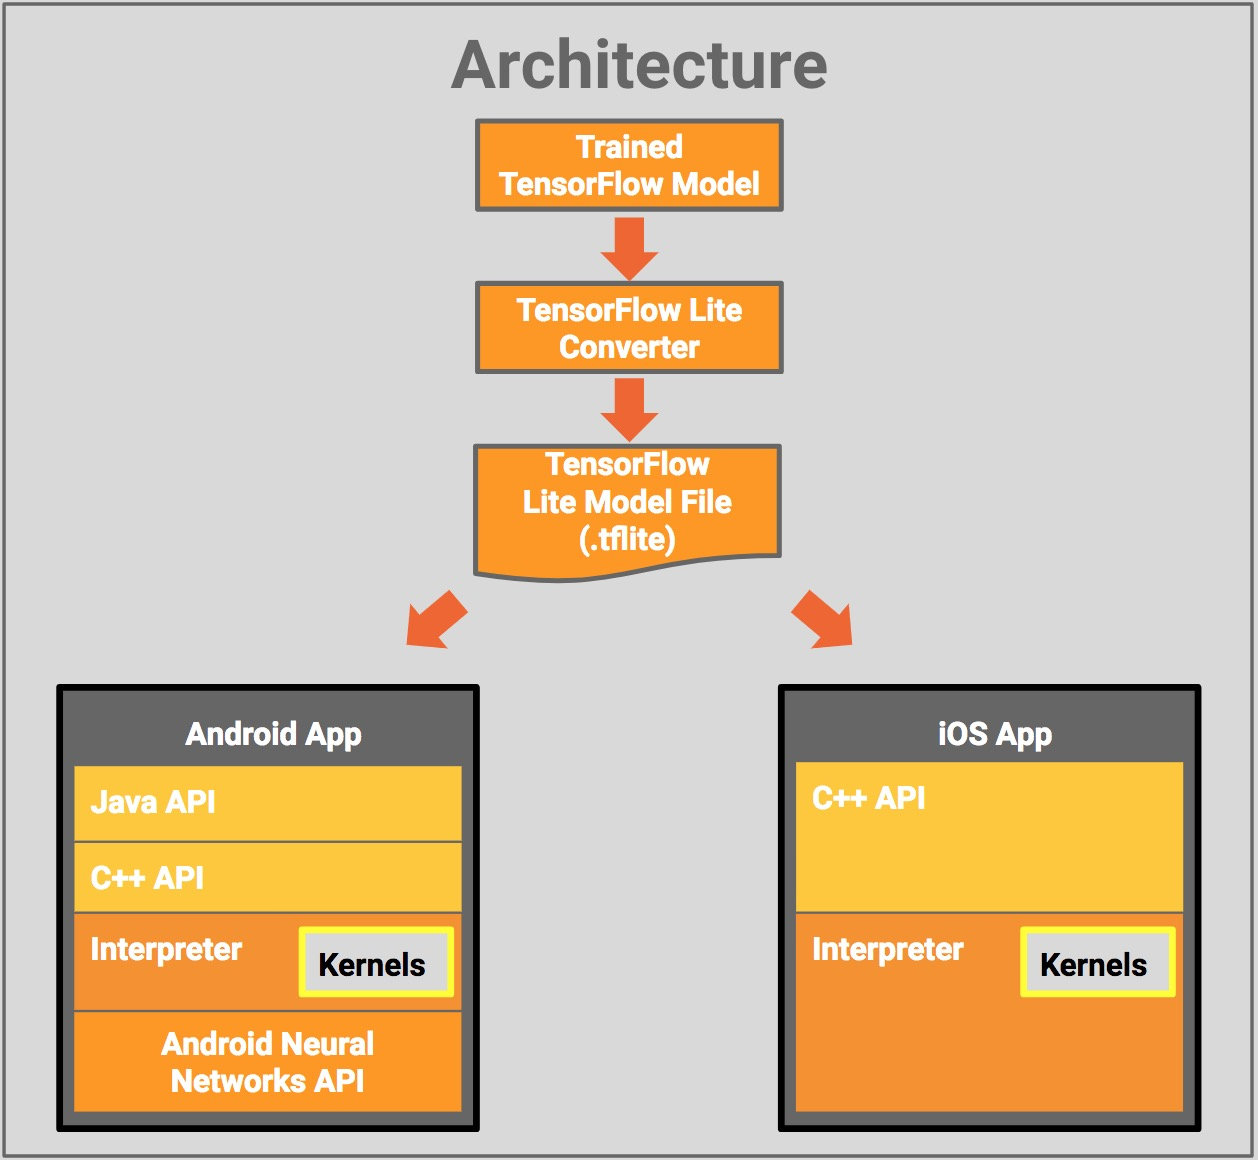
\includegraphics[width=0.75\textwidth]{architecture.jpg}
	\captionsource{TensorFlow Lite Architecture.}{\cite{archtflite}}
	\label{fig:tflite-architecture}
\end{figure}
%
%
\\The tools made available by TensorFLow Lite allow you to convert a model trained
on computing devices such as HPC clusters, the conversion operation supported by
a set of core operators, both quantized and float, which have been tuned for
mobile platforms. The core operations incorporated pre-fused activations and
biases to further enhance performance and quantized accuracy. 
TensorFlow Lite supports using custom operations in models. 
From this operation a more compact and better optimized model for portable
applications is obtained. This allows you to increase the speed of execution of
the model on devices such as Coral dev-Board, but not only.\\
The \texttt{.tflite} model is obtained from these commands which will perform
the quantization.
%
\begin{listing}[ht] 
\inputminted[frame=lines,framesep=2mm, linenos=true, autogobble, breaklines=true, fontsize=\scriptsize, firstline=16, lastline=46]{shell}{neuralnetworks/code/tflite_ssd_mobilenet_v2_coco_2018_03_29.sh} 
\caption{Train script setup.} 
\label{lst:tflite-code-shell} 
\end{listing}
%
\\The biggest advantage is obtained when the evaluation of the neural network
takes place as they involve numerous calculations that drastically affect the
energy consumption of the processor and consequently on the battery used to
power the device. 
The simplification of the model allows you to use less memory and cycles as it
is possible to switch from 32-bit floating point calculations to calculations
with 8-bit integers. 
This has repercussions on processors that have high performance and reduced
consumption.